\documentclass{article}
\PassOptionsToPackage{numbers, compress}{natbib}
\usepackage[main,final]{neurips_2026}
\usepackage[utf8]{inputenc}
\usepackage[T1]{fontenc}
\usepackage[hidelinks]{hyperref}
\usepackage{url}
\usepackage{booktabs}
\usepackage{amsmath}
\usepackage{graphicx}
\usepackage{microtype}
\usepackage{tikz}
\usetikzlibrary{positioning,arrows.meta,calc}

\title{Where the Penalty Goes: A Climate-Resolved Audit of\\ Transferable HVAC Control in the Smart Buildings Challenge}

\author{%
  Ahmad Dweikat\\
  Princess Sumaya University for Technology (PSUT)\\
  Amman, Jordan\\
  \texttt{ahmedhaz1414@gmail.com}
}

\begin{document}
\maketitle

\begin{abstract}
The NeurIPS 2026 Smart Buildings Challenge \cite{goldfeder2026} scores an HVAC controller on buildings and climates it has never seen, by a reward that mixes occupant comfort (weight 0.6), energy cost (0.2) and carbon (0.2). We ask which of the three terms a controller pays, in which climate, and at what time of day. On all 30 training scenarios (six buildings, five climates, 30 days each) under the corrected Round~2 simulator, we compare the strongest shipped baseline (\texttt{pid\_water}) with a strong public controller, CtrlX \cite{morev2026}, built on Wu's analytical controller \cite{wu2026}. (i) CtrlX is better in every scenario, by 4.7--29.1$\times$ (median 8.3$\times$). The baseline loses mainly on comfort (61\% of its score); CtrlX's comfort term is at most 5\% of its score in any scenario. (ii) What remains is energy and carbon; the cold climate alone is 42\% of CtrlX's total, 77\% of that cold-climate penalty is incurred while the building is occupied, and 92\% of the occupied-hours bill is gas, burned to reheat supply air that is at least 30\% outdoor air. (iii) Schedule ideas that help the baseline by up to 24\% are worth at most 0.1\% on CtrlX, and no single heating-parameter change improves it (the worst costs 0.3\%). (iv) Releasing zones once they empty in the afternoon would gain 5.3\% if a controller knew who sat where, but a person leaves only a weak trace in the sensors a submission sees (best AUC 0.63 on average), and a release rule built on that trace loses in all 30 scenarios: because comfort is averaged over the people present, one wrongly released zone late in the day costs far more than the right ones save. (v) A hot-water storage option that helped under the Round~1 simulator is worth nothing after the fix, both locally ($-0.08\%$) and on the hidden leaderboard (0.00984 vs.\ 0.00983). The remaining gap is heating an occupied building in cold weather, not scheduling, accounting or guessing who is present.
\end{abstract}

\section{Introduction}
Most building controllers are tuned to one building. The challenge asks for the opposite: one policy, evaluated on six unseen buildings $\times$ five unseen weather stations, 30 days each at five-minute steps. The per-step reward is
\[ r_t = 0.6\,p_t - 0.2\,c_t - 0.2\,e_t, \qquad r_t \le 0, \]
with $p_t$ an occupancy-weighted comfort regret, $c_t$ energy cost and $e_t$ carbon. The score is the mean of $-\bar r$ over scenarios; lower is better.

A single number hides why a controller is good. We report every result split into its three terms, by climate and by building state. The audit needs no new controller and answers a practical question for every team: \emph{where is the next unit of score?} Our contributions are:
\begin{itemize}
  \item a decomposition of the score of a weak and a strong transferable controller over all 30 training scenarios under the corrected simulator (Sec.~\ref{sec:anatomy});
  \item a time-of-day split showing that the remaining cold-climate penalty is spent while the building is occupied (Sec.~\ref{sec:when});
  \item an ablation and a sensitivity sweep showing that schedule ideas and parameter tuning no longer pay off on the strong controller (Secs.~\ref{sec:ablation}--\ref{sec:sweep});
  \item a test of the largest remaining lever, per-zone occupancy, on all 30 scenarios: a person leaves only a weak trace in the sensors a submission sees, and releasing zones on that trace loses in every scenario, while the same release on true occupancy wins in every scenario (Sec.~\ref{sec:occ});
  \item a before/after measurement of the Round~2 hot-water fix, locally and on the hidden leaderboard (Sec.~\ref{sec:accounting}).
\end{itemize}

\section{Related work}\label{sec:related}
\textbf{Learning and optimal control for HVAC.} Model predictive control is a widely studied advanced method for buildings; Drgo\v{n}a et al.\ \cite{drgona2020} survey its formulations and tools and point out that results from individual case studies are hard to compare. Deep reinforcement learning has been applied to HVAC since at least Wei et al.\ \cite{wei2017}, and Wang and Hong \cite{wang2020} review the field and find few deployments in real buildings. A controller trained for one building rarely works in another: Xu et al.\ \cite{xu2020} transfer a learned HVAC controller across buildings with different sizes, zones and climates by retraining part of the network. The challenge we study removes that retraining step altogether: a policy must work zero-shot on unseen buildings.

\textbf{Benchmarks.} BOPTEST \cite{blum2021} made control results comparable by fixing emulators and key performance indicators. The Smart Buildings Control Suite \cite{goldfeder2023,goldfeder2025}, on which the challenge simulator is built, adds lightweight calibrated simulators of real office buildings meant for training controllers at scale. Benchmarks report a single score; our contribution is to take one apart by term, climate and building state, and to show which parts of it a transferable controller can still change.

\textbf{Occupancy-driven control.} Conditioning only occupied space is a long-standing source of savings: Agarwal et al.\ \cite{agarwal2010} and Erickson and Cerpa \cite{erickson2010} used dedicated occupancy sensors (wireless motion sensors and a camera network) to drive HVAC schedules, and Ardakanian et al.\ \cite{ardakanian2016} estimated per-zone occupancy from the sensors a building management system already has, in order to cut reheat. Section~\ref{sec:occ} asks the same question under the challenge's rules, with only standard zone sensors and a building headcount, and finds that the reward's per-person comfort averaging makes a noisy estimate far more costly than in those settings.

\section{Setup}
\textbf{Simulator and scenarios.} We use the official starter kit with the Round~2 fixes (energy-balanced hot-water tank; return air mixed by airflow). The main results cover all 30 training scenarios (buildings \texttt{train\_1,2,4,5,7,8} $\times$ Atlanta, Denver, Fairbanks, Phoenix, Singapore), each a full 30-day episode (8{,}640 steps), run in a Kaggle notebook against the competition data. Ablations and sweeps use building \texttt{train\_1} in four climates with shorter episodes (14 days for \texttt{pid\_water}, 7 days for CtrlX); the occupancy study uses all 30 scenarios with 6- and 7-day episodes. The simulator is deterministic, so each number is one exact rollout.

\textbf{Controllers.}
\emph{pid\_water} is the strongest controller shipped with the starter kit: per-AHU PID loops with a hot-water reset.
\emph{Setback}, \emph{LeadOnly} and \emph{Combo} are our occupancy-aware layers on \texttt{pid\_water}: drop the heating floor to 283\,K while the building is empty; condition early before arrivals (long pre-cool, short pre-heat); or both.
\emph{CtrlX} \cite{morev2026} is a supervisory layer on Wu's analytical controller \cite{wu2026}, which identifies a thermal model per zone and searches feasible air-handler operating points. All controllers read only observations and building metadata: no building identifier, weather label or scenario lookup.

\section{Where the penalty goes}\label{sec:anatomy}

\begin{table}[t]
\centering
\caption{Mean score (lower is better) and its weighted terms over the six buildings of each climate; 30-day episodes, Round~2 simulator. Comfort $=0.6\,|p|$, energy $=0.2\,c$, carbon $=0.2\,e$.}
\label{tab:anatomy}
\small
\begin{tabular}{llrrrrr}
\toprule
Climate & Controller & Score & Comfort & Energy & Carbon & Ratio \\
\midrule
Atlanta & pid\_water & 0.0303 & 0.0228 & 0.0047 & 0.0028 & \\
          & CtrlX & 0.0043 & 0.0001 & 0.0025 & 0.0018 & 7.0$\times$ \\
Denver & pid\_water & 0.0376 & 0.0319 & 0.0034 & 0.0023 & \\
          & CtrlX & 0.0035 & 0.0001 & 0.0016 & 0.0017 & 10.9$\times$ \\
Fairbanks & pid\_water & 0.1011 & 0.0473 & 0.0212 & 0.0327 & \\
          & CtrlX & 0.0143 & 0.0001 & 0.0041 & 0.0101 & 7.1$\times$ \\
Phoenix & pid\_water & 0.0756 & 0.0476 & 0.0204 & 0.0076 & \\
          & CtrlX & 0.0066 & 0.0000 & 0.0051 & 0.0014 & 11.5$\times$ \\
Singapore & pid\_water & 0.0448 & 0.0273 & 0.0129 & 0.0047 & \\
          & CtrlX & 0.0055 & 0.0000 & 0.0045 & 0.0011 & 8.1$\times$ \\
\midrule
All 30 & pid\_water & 0.0579 & 0.0353 & 0.0125 & 0.0100 & \\
          & CtrlX & 0.0068 & 0.0001 & 0.0036 & 0.0032 & 8.5$\times$ \\
\bottomrule
\end{tabular}
\end{table}

\begin{figure}[t]
\centering
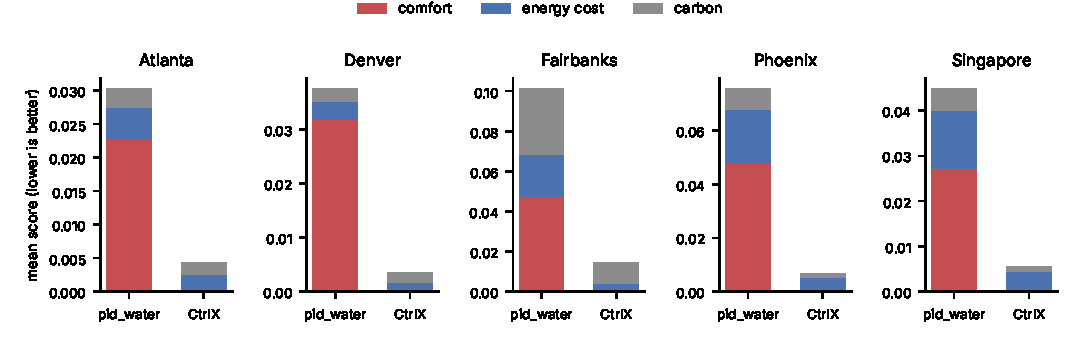
\includegraphics[width=\linewidth]{fig_anatomy.pdf}
\caption{Score anatomy per climate (mean of six buildings). The baseline pays mostly comfort; CtrlX pays almost only energy and carbon. Panels have different y-scales.}
\label{fig:anatomy}
\end{figure}

Table~\ref{tab:anatomy} and Fig.~\ref{fig:anatomy} show the decomposition.

\textbf{The baseline loses on comfort; the strong controller does not.} Comfort is 61\% of the \texttt{pid\_water} score summed over the 30 scenarios. CtrlX is better in every one of the 30 scenarios, by 4.7--29.1$\times$ (median 8.3$\times$, 8.5$\times$ on the mean score), and its comfort term never exceeds 5\% of its score in any scenario. Since comfort carries weight 0.6 and grows quadratically far outside the band, the largest leaderboard gains come from keeping every occupied zone in band, not from saving energy.

\textbf{What is left is energy and carbon, concentrated in the cold.} Summed over all scenarios, CtrlX's score is 52\% energy cost and 47\% carbon. Fairbanks accounts for 42\% of its total, and within Fairbanks carbon from gas heating is 71\% of the score. Any further honest improvement must deliver the same comfort with less heat in deep cold.

\section{When the cold-climate penalty is spent}\label{sec:when}
We split CtrlX's Fairbanks penalty (building \texttt{train\_1}, 7 days) by building state at each step: \emph{occupied} (occupants present), \emph{pre-arrival} (the schedule's comfort mode is about to start) and \emph{empty}. Occupied steps are 31\% of the time but 77\% of the penalty; pre-arrival is 10\% of the time and 12\% of the penalty; empty periods are 59\% of the time and only 11\% of the penalty. Night and weekend setback therefore has little left to save: the cost is heating the building while people are in it.

\begin{figure}[t]
\centering
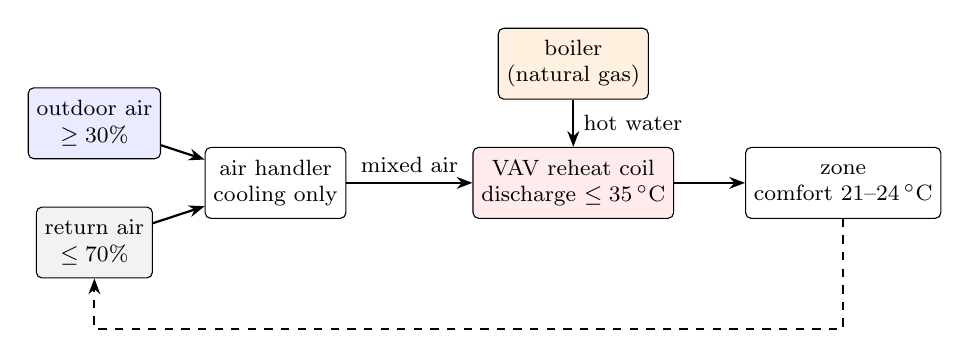
\begin{tikzpicture}[font=\footnotesize, node distance=6mm and 9mm,
  box/.style={draw, rounded corners=2pt, align=center, minimum height=9mm, inner sep=3pt},
  arr/.style={-{Stealth[length=2mm]}, thick}]
\node[box, fill=blue!8] (oa) {outdoor air\\$\ge 30\%$};
\node[box, fill=gray!10, below=of oa] (ra) {return air\\$\le 70\%$};
\node[box, right=14mm of $(oa)!0.5!(ra)$] (ahu) {air handler\\cooling only};
\node[box, fill=red!8, right=16mm of ahu] (vav) {VAV reheat coil\\discharge $\le 35\,^\circ$C};
\node[box, right=of vav] (zone) {zone\\comfort 21--24\,$^\circ$C};
\node[box, fill=orange!12, above=of vav] (boiler) {boiler\\(natural gas)};
\draw[arr] (oa) -- (ahu); \draw[arr] (ra) -- (ahu);
\draw[arr] (ahu) -- node[above]{mixed air} (vav);
\draw[arr] (boiler) -- node[right]{hot water} (vav);
\draw[arr] (vav) -- (zone);
\draw[arr, dashed] (zone.south) |- ++(0,-14mm) -| (ra.south);
\end{tikzpicture}
\caption{The only heating path in the simulator. Every supply stream carries at least 30\% outdoor air; the air handler can only cool, so all heat comes from gas burned in the boiler and delivered by the zone reheat coils, which are capped at a 35\,$^\circ$C discharge. In deep cold much of that gas only warms the outdoor share of the air back to the comfort band.}\label{fig:path}
\end{figure}

\textbf{Where that heat comes from.} Figure~\ref{fig:path} shows the only heating path. Splitting the occupied-hours energy bill by carrier, 92\% is natural gas. In the simulator, gas is burned only by the boiler that supplies the zone reheat coils; the air handlers can cool but have no heating branch, so there is no cheaper electric path for heat. The simulator also caps recirculation at 70\%, which forces at least 30\% outdoor air into every supply stream. In deep cold that outdoor air reaches each zone far below the comfort band and must be reheated with gas. CtrlX already keeps airflow near its minimum and prices gas explicitly when it chooses it; consistent with this, increasing or decreasing its gas weight (0.7--2$\times$) changed the score by at most 0.04\% (a 2$\times$ gas weight also scores 0.00983 on the hidden leaderboard, identical to CtrlX), and online re-identification of the thermal model made it 0.2\% worse (Round~2 simulator, four scenarios, 7 days). The remaining cold-climate penalty is largely set by the ventilation requirement, not by the controller.

\section{Ideas that help a weak controller do not transfer}\label{sec:ablation}

\begin{table}[t]
\centering
\caption{Change in score from schedule ideas, relative to the controller they are added to (building \texttt{train\_1}, Round~2 simulator; negative is better). \texttt{pid\_water} rows: 14-day episodes; CtrlX rows: 7-day episodes.}
\label{tab:ablation}
\small
\begin{tabular}{llrrrr}
\toprule
Base & Added idea & Phoenix & Denver & Fairbanks & Singapore \\
\midrule
pid\_water & Setback        & $-5.8\%$ & $-2.3\%$ & $-12.8\%$ & $+28.0\%$ \\
pid\_water & LeadOnly       & $-24.3\%$ & $-2.3\%$ & $+1.1\%$ & $-11.1\%$ \\
pid\_water & Combo          & $-24.4\%$ & $-1.6\%$ & $-15.9\%$ & $-11.1\%$ \\
\midrule
CtrlX & early pre-cool          & $-0.1\%$ & $0.0\%$ & $0.0\%$ & $+0.2\%$ \\
CtrlX & arrival lead 1 h        & $0.0\%$ & $+3.0\%$ & $+0.5\%$ & $0.0\%$ \\
CtrlX & free-air pre-cool       & $0.0\%$ & $0.0\%$ & $0.0\%$ & $0.0\%$ \\
\bottomrule
\end{tabular}
\end{table}

On \texttt{pid\_water}, conditioning before arrivals cuts the Phoenix and Singapore scores by 11--24\% (Table~\ref{tab:ablation}). Letting the empty building drift (Setback) helps in Fairbanks under the corrected simulator but costs 28\% in Singapore, where the morning recovery outweighs the night saving. On CtrlX the same ideas are worth at most 0.1\%, and a longer arrival lead costs up to 3\%: it already starts each zone when its own thermal model says it is needed. Improvements must be measured on a strong base; a result on the shipped baseline says little about the leaderboard.

\section{The strong controller is at an optimum}\label{sec:sweep}
We varied CtrlX's heating-side parameters one at a time on 7-day episodes in four climates (Round~2 simulator): comfort margin (0.04, 0.12 vs.\ 0.08\,K), heating response scale (0.65, 0.85 vs.\ 0.75), and hot-water ceiling and floor (345\,K; 325\,K). No change improved the four-climate total at all (the best was a tie); the worst cost 0.3\% (Table~\ref{tab:sweep}).

\textbf{How close to optimal?} Our sweep agrees with the CtrlX author's own records \cite{morev2026}: more than forty mechanisms tried on CtrlX (start-time rules, per-zone margins, hot-water strategies, air-handler duty cycling, forecast preheating, occupancy inference and two automated parameter searches) are logged as flat or worse, and an exact open-loop optimum computed on a differentiable copy of the simulator is reported to be only about 0.16\% better at matched comfort. The plant also sits on its device limits whenever it heats: 30\% outdoor air, minimum damper and static pressure, and reheat discharge at its 35\,$^\circ$C cap. At that cap the gas burned per watt of heat delivered to a zone no longer depends on airflow, so no pressure or damper setting can lower it; only when the plant runs, and how warm the zones are held while it runs, can.

\begin{table}[t]
\centering
\caption{One-at-a-time sensitivity of CtrlX, 7-day episodes, change in four-climate total (Round~2 simulator).}
\label{tab:sweep}
\small
\begin{tabular}{lr}
\toprule
Change & Total vs.\ CtrlX \\
\midrule
hot-water floor 325\,K & $0.00\%$ \\
comfort margin 0.04\,K & $+0.04\%$ \\
heating response 0.85 & $+0.02\%$ \\
hot-water ceiling 345\,K & $+0.05\%$ \\
comfort margin 0.12\,K & $+0.25\%$ \\
heating response 0.65 & $+0.29\%$ \\
\bottomrule
\end{tabular}
\end{table}

\section{Who is in which zone is only weakly observable}\label{sec:occ}
The largest remaining lever is per-zone occupancy: an oracle that releases each zone once it empties after noon is worth about 2.3\% on CtrlX's predecessor CtrlW \cite{morev2026}. A submission sees only the building-wide headcount \texttt{num\_occupants}. Two facts limit what it can do with that. First, comfort regret is normalised by the number of people present, so the comfort cost of relaxing every zone by one kelvin is the same whether one person or seventy remain; a headcount-scaled relaxation therefore buys nothing that a fixed margin does not, and CtrlX's margin is already optimal (Section~\ref{sec:sweep}). 

Second, the only per-zone trace of a person in the simulator is 70\,W of sensible heat, which changes zone temperatures under CtrlX by 0.07\,K on average. We tested whether that trace is visible in all 30 training scenarios (6-day episodes, 13:00--19:00, occupancy redrawn every day), comparing occupied and empty zones within the same hour of day. Each single signal separates them only weakly (Figure~\ref{fig:occ}a): the best of zone temperature, damper command and a per-zone model residual reaches a mean AUC of 0.63 (range 0.53--0.81; 0.5 is chance). The signal is strongest in warm climates, where occupied zones call for more cooling air (damper AUC 0.70 in Singapore, 0.63 in Phoenix), and weakest in cold ones (best 0.58 in Fairbanks), where the oracle's gain is largest. 

\textbf{Acting on the estimate.} Is that enough to act on? We built a release rule on CtrlX: a logistic estimator over causal, per-zone standardised versions of the three signals (trained on four \texttt{train\_1} episodes) ranks the zones each afternoon step, and the $n_\text{zones}-\lceil N\rceil$ lowest-ranked zones, where $N$ is the headcount (so at least that many zones are truly empty), are released. Table~\ref{tab:occ} compares it with the same release driven by true occupancy and by a random ranking. True occupancy saves 4.6\% in Phoenix and 1.0\% in Fairbanks; the estimator loses 101\% and 14\%, no better than random. Across all 30 training scenarios (Figure~\ref{fig:occ}b; 7-day episodes; 26 of them on buildings the estimator never saw), true-occupancy release improves CtrlX in every scenario (mean $-5.3\%$, range $-1.0$ to $-13.2\%$), while the estimator-driven 1\,K release is worse in every scenario (mean $+187\%$, range $+14$ to $+818\%$). Each wrongly released zone usually holds one of the last few people in the building, and because regret is averaged over the people present, the wrong releases cost an order of magnitude more comfort than the right ones save in energy. A release rule therefore needs near-perfect precision, which an AUC of 0.6--0.8 cannot give: the 2.3\% oracle gain stays out of reach.

\begin{figure}[t]
\centering
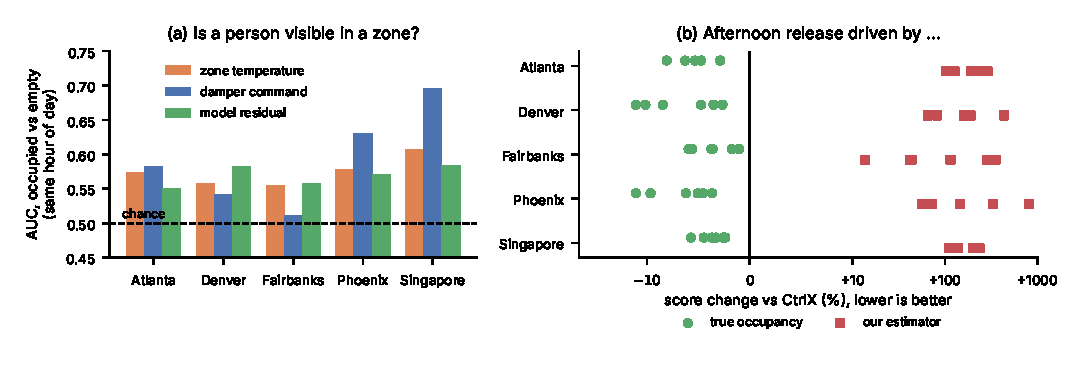
\includegraphics[width=\linewidth]{fig_occ.pdf}
\caption{Per-zone occupancy across the 30 training scenarios (Round~2 simulator, CtrlX). (a)~How well each sensor signal separates occupied from empty zones in the same afternoon hour, averaged per climate. (b)~Score change from releasing zones in the afternoon, one point per scenario: driven by true occupancy (analysis only) and by our estimator with a 1\,K release. The axis is linear within $\pm10\%$ and logarithmic beyond.}\label{fig:occ}
\end{figure}

\begin{table}[h]
\centering\small
\caption{Afternoon per-zone release on CtrlX, 7-day episodes on \texttt{train\_1}, Round~2 simulator (score, lower is better; change vs CtrlX). ``1\,K'' lowers the released zones' band by 1\,K instead of dropping it to standby.}\label{tab:occ}
\begin{tabular}{lrrrr}
\toprule
& \multicolumn{2}{c}{Phoenix} & \multicolumn{2}{c}{Fairbanks}\\
release driven by & score & $\Delta$ & score & $\Delta$\\
\midrule
none (CtrlX) & 0.01209 & --- & 0.04146 & ---\\
true occupancy & 0.01154 & $-4.6\%$ & 0.04103 & $-1.0\%$\\
true occupancy, 1\,K & 0.01167 & $-3.5\%$ & & \\
estimator & 0.02433 & $+101\%$ & & \\
estimator, 1\,K & 0.01886 & $+56\%$ & 0.04707 & $+13.5\%$\\
random ranking & 0.02218 & $+83\%$ & & \\
random ranking, 1\,K & 0.01849 & $+53\%$ & & \\
\bottomrule
\end{tabular}
\end{table}

\section{The Round~2 hot-water fix, before and after}\label{sec:accounting}
CtrlX ships an optional \emph{tank hold} that keeps the hot-water reservoir charged between demand peaks. Its author reports that it partly exploited how the Round~1 simulator billed boiler energy \cite{morev2026}. After the fix, tank hold changes CtrlX's four-climate total by $-0.08\%$ locally (removing it is marginally better), and on the hidden public leaderboard our submissions with and without it score 0.00984 and 0.00983. CtrlX itself is almost unaffected by the fix (four-climate total 0.07217 before, 0.07236 after, $+0.3\%$), whereas participants report the unchanged \texttt{pid\_water} baseline moving from 0.06404 to 0.07414. CtrlX's gains are therefore physical, not an artifact of billing.

\section{Limitations}
The ablation, the time-of-day split and the sweep use one building and shorter episodes (7 or 14 days). We studied one strong controller; the sweep was one-at-a-time and cannot rule out gains from changing several parameters together. Our occupancy estimator is a linear model trained on four episodes; a better estimator could separate zones more sharply, but Table~\ref{tab:occ} shows the bar it must clear is near-perfect precision, not a modest AUC gain. Rankings on the hidden buildings may differ from the training set.

\section{Conclusion}
Splitting the challenge score by term, climate and building state shows where controllers stand. The shipped baseline loses on comfort; a strong transferable controller removes that loss in every training scenario, and what remains is heat in cold weather, spent while the building is occupied. Schedule ideas that look large on a weak base vanish on a strong one, the strong controller's parameters are already optimal, and the Round~2 fix confirms that its savings are physical. Per-zone occupancy, the one lever with a measured upside, is only weakly visible in the observations a submission receives, and acting on a weak estimate costs far more than it saves, because the last people in a building carry the whole comfort term. The next gain must come from conditioning occupied, cold buildings with less heat, not from tuning schedules or guessing who is present.

\paragraph{Code and data.} All controllers, run scripts, notebooks and per-scenario results are available from the author. CtrlX and Wu's controller are used under the Apache-2.0 license.

\small
\begin{thebibliography}{99}
\bibitem{agarwal2010} Y.~Agarwal, B.~Balaji, R.~Gupta, J.~Lyles, M.~Wei, and T.~Weng. Occupancy-driven energy management for smart building automation. In \emph{BuildSys}, pages 1--6, 2010.
\bibitem{ardakanian2016} O.~Ardakanian, A.~Bhattacharya, and D.~Culler. Non-intrusive techniques for establishing occupancy related energy savings in commercial buildings. In \emph{BuildSys}, pages 21--30, 2016.
\bibitem{blum2021} D.~Blum, J.~Arroyo, S.~Huang, J.~Drgo\v{n}a, F.~Jorissen, H.~T.~Walnum, Y.~Chen, K.~Benne, D.~Vrabie, M.~Wetter, and L.~Helsen. Building optimization testing framework ({BOPTEST}) for simulation-based benchmarking of control strategies in buildings. \emph{Journal of Building Performance Simulation}, 14(5):586--610, 2021.
\bibitem{drgona2020} J.~Drgo\v{n}a, J.~Arroyo, I.~Cupeiro Figueroa, D.~Blum, K.~Arendt, D.~Kim, E.~Perarnau Oll\'e, J.~Oravec, M.~Wetter, D.~L.~Vrabie, and L.~Helsen. All you need to know about model predictive control for buildings. \emph{Annual Reviews in Control}, 50:190--232, 2020.
\bibitem{erickson2010} V.~L.~Erickson and A.~E.~Cerpa. Occupancy based demand response {HVAC} control strategy. In \emph{BuildSys}, 2010.
\bibitem{goldfeder2023} J.~Goldfeder and J.~Sipple. A lightweight calibrated simulation enabling efficient offline learning for optimal control of real buildings. \emph{arXiv:2310.08569}, 2023.
\bibitem{goldfeder2025} J.~Goldfeder, V.~Dean, Z.~Jiang, X.~Wang, B.~Dong, H.~Lipson, and J.~Sipple. The Smart Buildings Control Suite: a diverse open source benchmark to evaluate and scale {HVAC} control policies for sustainability. \emph{arXiv:2410.03756}, 2025.
\bibitem{goldfeder2026} J.~Goldfeder et al. Smart Buildings Competition. Kaggle, 2026. \url{https://www.kaggle.com/competitions/neurips-2026-smart-buildings}.
\bibitem{morev2026} S.~Morev. Stop heating an empty building: reward anatomy and a supervisory layer for the NeurIPS 2026 Smart Buildings Challenge. Round-1 paper, 2026. \url{https://github.com/MorS1337/sb26-stop-heating}.
\bibitem{wang2020} Z.~Wang and T.~Hong. Reinforcement learning for building controls: the opportunities and challenges. \emph{Applied Energy}, 269:115036, 2020.
\bibitem{wei2017} T.~Wei, Y.~Wang, and Q.~Zhu. Deep reinforcement learning for building {HVAC} control. In \emph{Design Automation Conference (DAC)}, 2017.
\bibitem{wu2026} D.~Wu. CPU A -- alpha 0.75 control. Kaggle notebook, 2026. \url{https://www.kaggle.com/code/danielwuu/cpu-a-alpha075-control-20261022}.
\bibitem{xu2020} S.~Xu, Y.~Wang, Y.~Wang, Z.~O'Neill, and Q.~Zhu. One for many: transfer learning for building {HVAC} control. In \emph{BuildSys}, pages 230--239, 2020.
\end{thebibliography}

\end{document}
